% Options for packages loaded elsewhere
\PassOptionsToPackage{unicode}{hyperref}
\PassOptionsToPackage{hyphens}{url}
%
\documentclass[
]{article}
\usepackage{amsmath,amssymb}
\usepackage{iftex}
\ifPDFTeX
  \usepackage[T1]{fontenc}
  \usepackage[utf8]{inputenc}
  \usepackage{textcomp} % provide euro and other symbols
\else % if luatex or xetex
  \usepackage{unicode-math} % this also loads fontspec
  \defaultfontfeatures{Scale=MatchLowercase}
  \defaultfontfeatures[\rmfamily]{Ligatures=TeX,Scale=1}
\fi
\usepackage{lmodern}
\ifPDFTeX\else
  % xetex/luatex font selection
\fi
% Use upquote if available, for straight quotes in verbatim environments
\IfFileExists{upquote.sty}{\usepackage{upquote}}{}
\IfFileExists{microtype.sty}{% use microtype if available
  \usepackage[]{microtype}
  \UseMicrotypeSet[protrusion]{basicmath} % disable protrusion for tt fonts
}{}
\makeatletter
\@ifundefined{KOMAClassName}{% if non-KOMA class
  \IfFileExists{parskip.sty}{%
    \usepackage{parskip}
  }{% else
    \setlength{\parindent}{0pt}
    \setlength{\parskip}{6pt plus 2pt minus 1pt}}
}{% if KOMA class
  \KOMAoptions{parskip=half}}
\makeatother
\usepackage{xcolor}
\usepackage[margin=1in]{geometry}
\usepackage{graphicx}
\makeatletter
\def\maxwidth{\ifdim\Gin@nat@width>\linewidth\linewidth\else\Gin@nat@width\fi}
\def\maxheight{\ifdim\Gin@nat@height>\textheight\textheight\else\Gin@nat@height\fi}
\makeatother
% Scale images if necessary, so that they will not overflow the page
% margins by default, and it is still possible to overwrite the defaults
% using explicit options in \includegraphics[width, height, ...]{}
\setkeys{Gin}{width=\maxwidth,height=\maxheight,keepaspectratio}
% Set default figure placement to htbp
\makeatletter
\def\fps@figure{htbp}
\makeatother
\setlength{\emergencystretch}{3em} % prevent overfull lines
\providecommand{\tightlist}{%
  \setlength{\itemsep}{0pt}\setlength{\parskip}{0pt}}
\setcounter{secnumdepth}{5}
\ifLuaTeX
  \usepackage{selnolig}  % disable illegal ligatures
\fi
\usepackage[]{natbib}
\bibliographystyle{plainnat}
\usepackage{bookmark}
\IfFileExists{xurl.sty}{\usepackage{xurl}}{} % add URL line breaks if available
\urlstyle{same}
\hypersetup{
  pdftitle={Descrição das etapas de processamento de dados de inventário realizado com o auxílio da tecnologia LiDAR},
  pdfauthor={Otávio Magalhães Silva Souza},
  hidelinks,
  pdfcreator={LaTeX via pandoc}}

\title{Descrição das etapas de processamento de dados de inventário
realizado com o auxílio da tecnologia LiDAR}
\author{Otávio Magalhães Silva Souza}
\date{}

\begin{document}
\maketitle

\begin{center}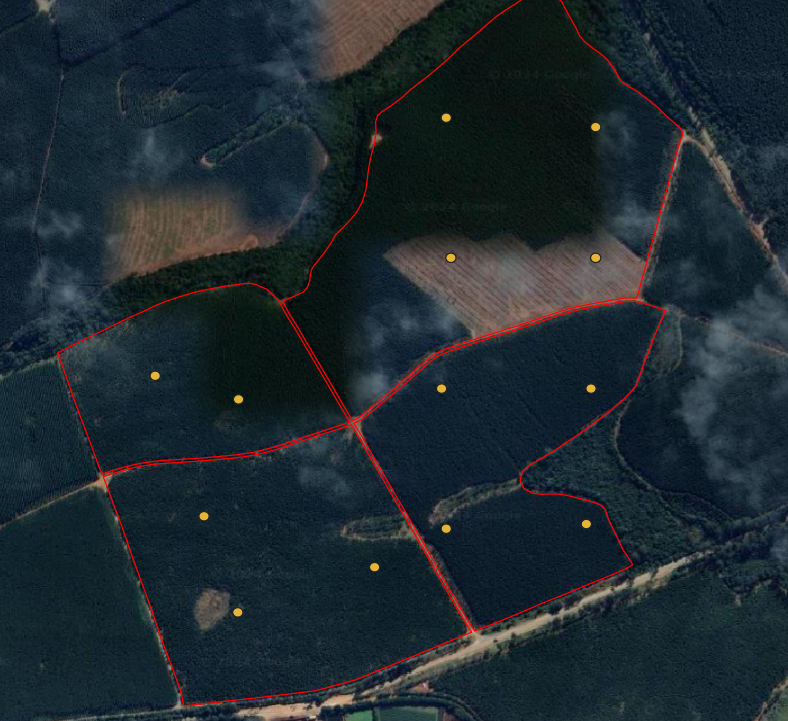
\includegraphics[width=0.4\linewidth]{IMAGES/CAPA} \end{center}

\centerline {Piracicaba, SP – Data de Emissão: 23 de julho de 2024}
\newpage

\tableofcontents

\newpage

\section{Pacotes utilizados no R (colocar breve descrição - já tem uma
descriçãozinha no R passado em
aula)}\label{pacotes-utilizados-no-r-colocar-breve-descriuxe7uxe3o---juxe1-tem-uma-descriuxe7uxe3ozinha-no-r-passado-em-aula}

\subsection{\texorpdfstring{Tidyverse
(\url{https://livro.curso-r.com/4-2-tidyverse.html})}{Tidyverse (https://livro.curso-r.com/4-2-tidyverse.html)}}\label{tidyverse-httpslivro.curso-r.com4-2-tidyverse.html}

O Tidyverse é um pacote guarda-chuva e contém diversas funções úteis
para garantir o dinamismo no script, visualização, processamento e
análise dos dados, modelagem etc.

\begin{figure}

{\centering 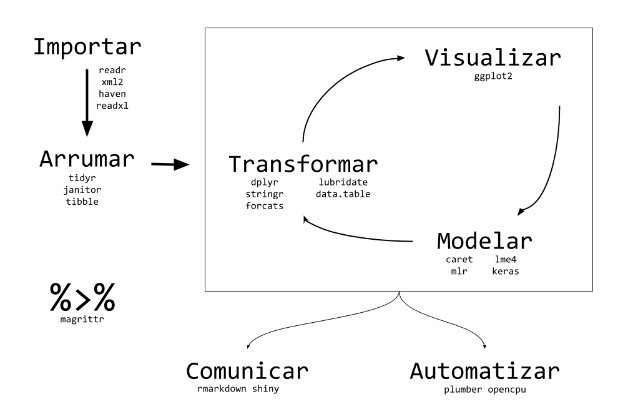
\includegraphics[width=0.6\linewidth]{IMAGES/tidyverse} 

}

\caption{Tidyverse}\label{fig:unnamed-chunk-2}
\end{figure}

\subsection{Sf}\label{sf}

Pacote utilizado para manipulação de objetos do mundo real. Descreve a
forma com que esses objetos podem ser armazenados e importados e quais
operações geométricas podem ser definidas por eles.

\subsection{Tidyterra}\label{tidyterra}

\subsection{Terra}\label{terra}

\subsection{Stars}\label{stars}

\subsection{Tools}\label{tools}

\subsection{RColorBrewer}\label{rcolorbrewer}

\subsection{Progress}\label{progress}

\subsection{Reshape2}\label{reshape2}

\subsection{Mapview}\label{mapview}

\subsection{LidR}\label{lidr}

\subsection{RCSF}\label{rcsf}

\subsection{Future}\label{future}

\newpage

\section{Descrição da área}\label{descriuxe7uxe3o-da-uxe1rea}

A área a ser estudada como ``Fazenda Modelo'' localiza-se no município
de São Miguel Arcanjo (SP), pode ser identificada pelas coordenadas
(-23.86707°, -47.87772°) e possui 129,784 ha, que dividem-se em 4
subtalhões: 301a (18,933 ha), 301d (34,468 ha), 302a (47,602 ha) e 302c
(28,781 ha).

\begin{figure}

{\centering 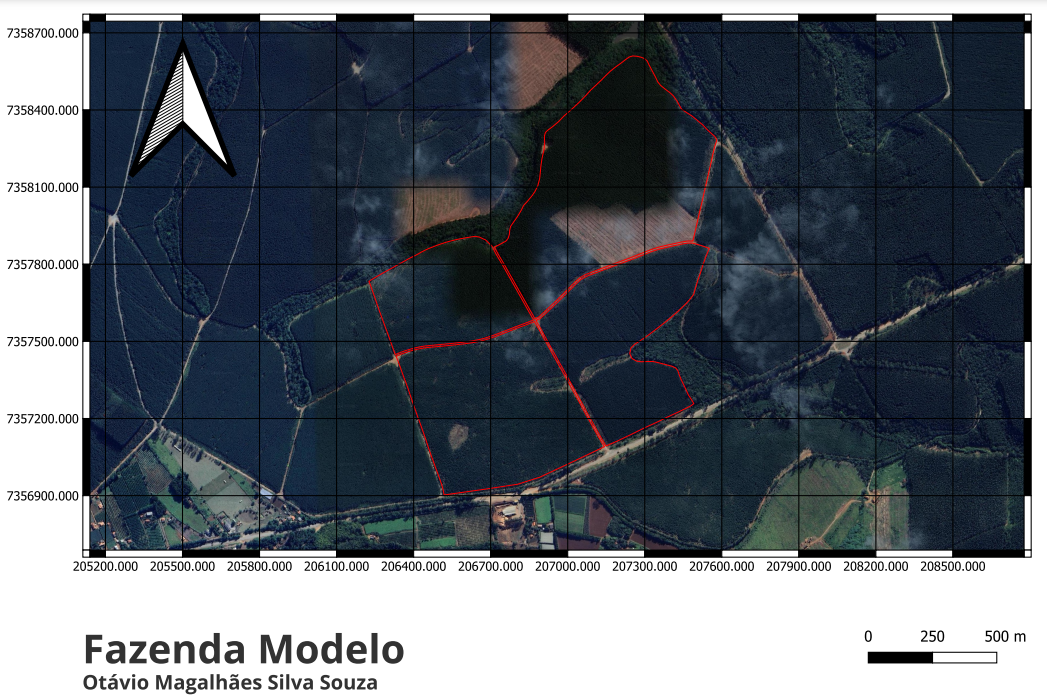
\includegraphics[width=0.6\linewidth]{IMAGES/mapafazendamodelo} 

}

\caption{Mapa da propriedade}\label{fig:unnamed-chunk-3}
\end{figure}
\begin{figure}

{\centering 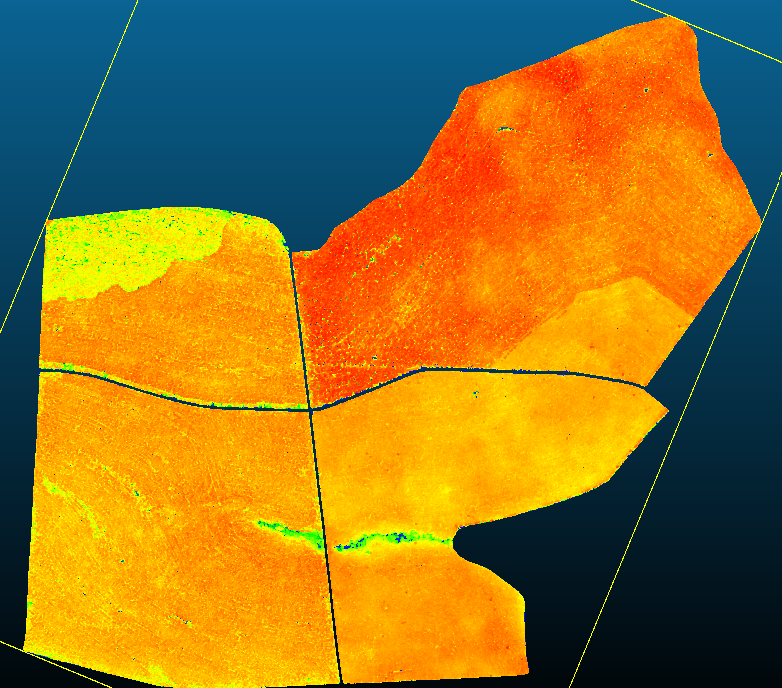
\includegraphics[width=0.4\linewidth]{IMAGES/nuvensnormalizadas} 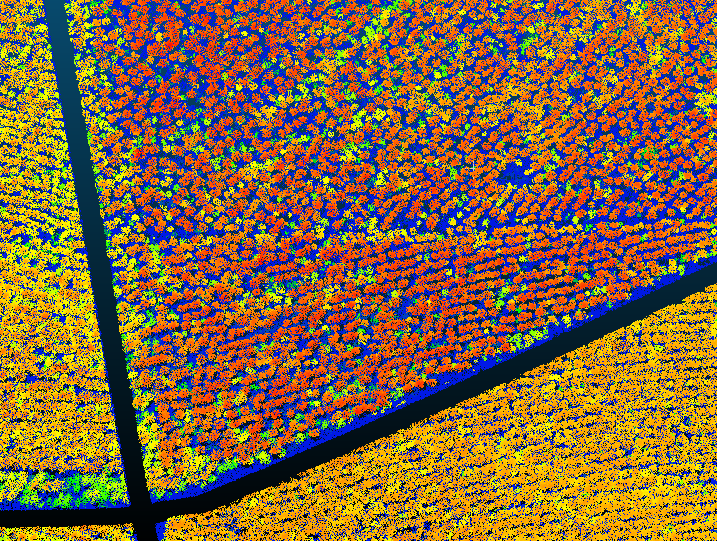
\includegraphics[width=0.4\linewidth]{IMAGES/nuvensnormalizadaszoom} 

}

\caption{Nuvens LiDAR normalizadas}\label{fig:unnamed-chunk-4}
\end{figure}

\newpage

\section{Grid e parcelas já
inventariadas}\label{grid-e-parcelas-juxe1-inventariadas}

A região foi dividida em 3454 parcelas, onde 2960 delas possuem 400m²,
enquanto as outras são menores por estarem na borda e abrangerem áreas
além da área de interesse. Além disso, 13 das parcelas possuem dados de
inventário florestal e podem ser identificadas pelos seguintes Id's:
993, 1526, 1770, 1881, 3165, 3628, 3660, 3730, 5052, 5091, 5106 e 5122.

\begin{figure}

{\centering 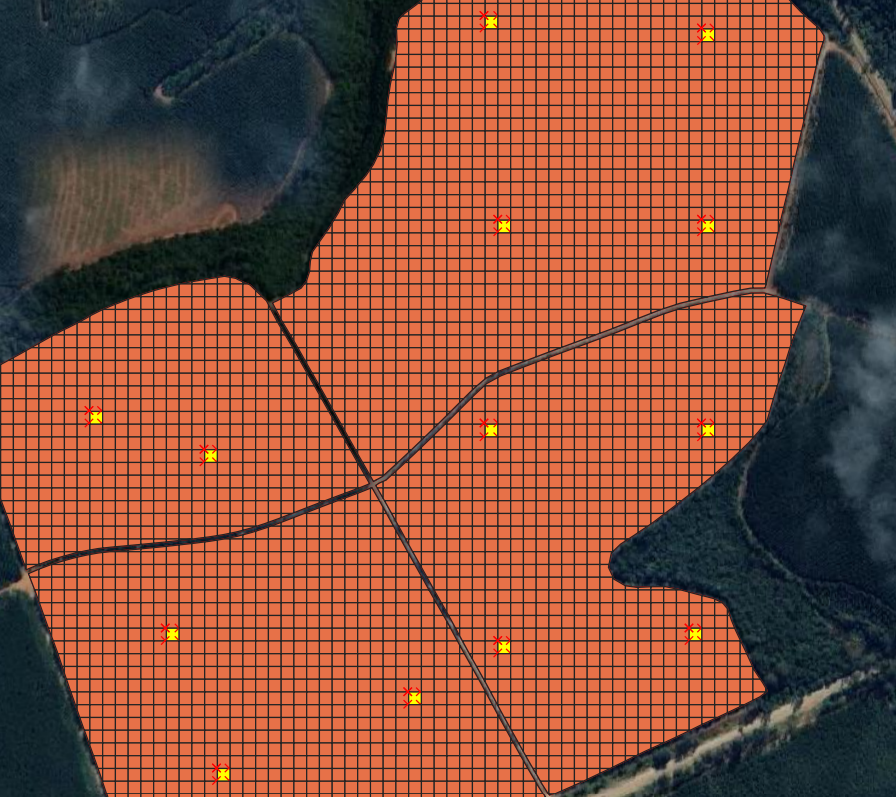
\includegraphics[width=0.4\linewidth]{IMAGES/parcelasinventariadas} 

}

\caption{Parcelas com dados de inventário}\label{fig:unnamed-chunk-5}
\end{figure}
\newpage

\section{Fluxograma e etapas Dupla
amostragem}\label{fluxograma-e-etapas-dupla-amostragem}

\begin{figure}

{\centering 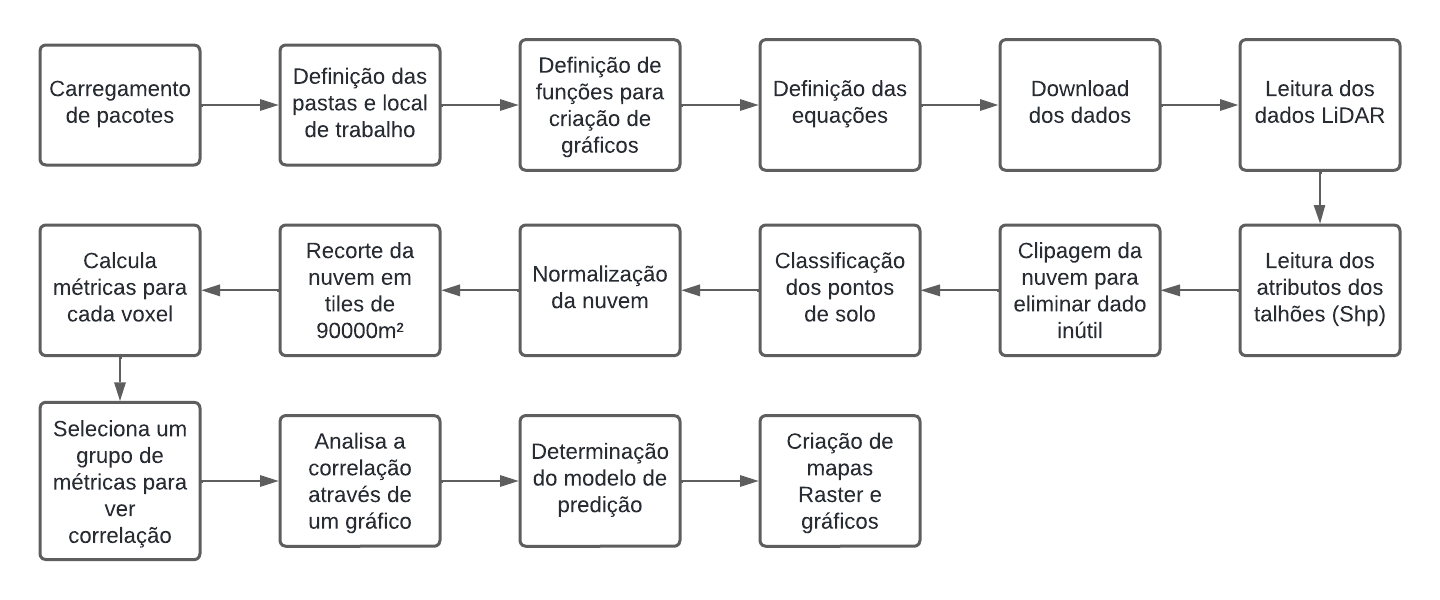
\includegraphics[width=0.8\linewidth]{IMAGES/fluxogramaDA} 

}

\caption{Fluxograma das etapas de processamento de dados LiDAR para fins de inventário florestal}\label{fig:unnamed-chunk-6}
\end{figure}

\begin{enumerate}
\def\labelenumi{\arabic{enumi}.}
\tightlist
\item
  Carregamento dos pacotes
\end{enumerate}

\begin{enumerate}
\def\labelenumi{\roman{enumi}.}
\tightlist
\item
  Diversos são os pacotes carregados. Os nomes e a utilidade de cada um
  estão descritos na primeira seção do documento. \newpage
\end{enumerate}

\begin{enumerate}
\def\labelenumi{\arabic{enumi}.}
\setcounter{enumi}{1}
\tightlist
\item
  Definição das pastas e local de trabalho
\end{enumerate}

\begin{itemize}
\tightlist
\item
  GitHub

  \begin{enumerate}
  \def\labelenumi{\roman{enumi}.}
  \tightlist
  \item
    C: - pasta raiz
  \item
    GitRepo - diretório em que estão agrupados os arquivos a serem
    upados no GitHub
  \item
    PRJ\_FAZENDAMODELO - pasta do projeto
  \item
    RMD - código e arquivos utilizados na redação do presente documento
  \item
    RESULTADOS - plot da matriz de correlação
  \item
    BATCHR - arquivo tipo R com os scripts utilizados no pré e
    pós-processamento dos dados
  \item
    SAIDASSIG - arquivos gerados no QGIS
  \item
    SHAPES - arquivos de entrada para uso no SIG
  \end{enumerate}
\item
  LiDAR

  \begin{enumerate}
  \def\labelenumi{\roman{enumi}.}
  \tightlist
  \item
    C: - pasta raiz
  \item
    LiDAR - agrupa todos as nuvens de pontos utilizadas no script
  \item
    PRJ\_FAZENDAMODELO - pasta do projeto
  \item
    NUVENS - onde se localizam as nuvens de pontos
  \item
    A13 - reúne as nuvens do ano de 2013
  \item
    TALHOES - nuvem segregada por talhão
  \item
    NoNORM - nuvens com solo classificado
  \item
    SiNORM - nuvens com solo classificado e normalizadas
  \item
    RSTR\_qua - raster apresentando a estimativa da variável de
    interesse para cada talhão
  \end{enumerate}
\end{itemize}

\begin{figure}

{\centering 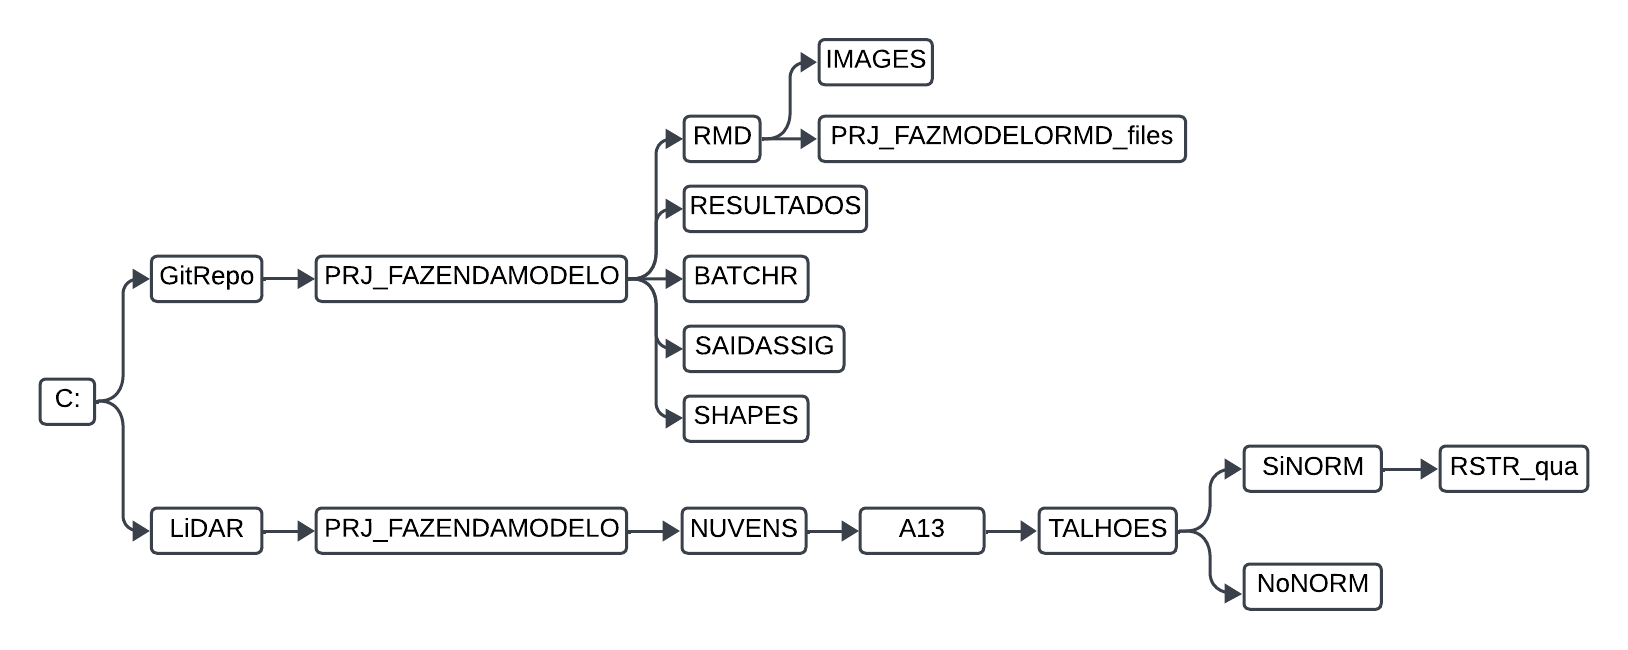
\includegraphics[width=0.8\linewidth]{IMAGES/organizacao-pastas} 

}

\caption{Organização dos diretórios}\label{fig:unnamed-chunk-7}
\end{figure}
\newpage

\begin{enumerate}
\def\labelenumi{\arabic{enumi}.}
\setcounter{enumi}{2}
\tightlist
\item
  Definição das funções para criação dos gráficos
\end{enumerate}

\newpage

\begin{enumerate}
\def\labelenumi{\arabic{enumi}.}
\setcounter{enumi}{3}
\tightlist
\item
  Definição das equações (estudar quais são)
\end{enumerate}

\newpage

\begin{enumerate}
\def\labelenumi{\arabic{enumi}.}
\setcounter{enumi}{4}
\tightlist
\item
  Download e leitura dos dados LiDAR
\end{enumerate}

\begin{enumerate}
\def\labelenumi{\roman{enumi}.}
\tightlist
\item
  Ao todo foram baixadas 6 nuvens de pontos LiDAR, que antes do
  processamento encontravam-se da seguinte maneira:
\end{enumerate}

\begin{figure}

{\centering 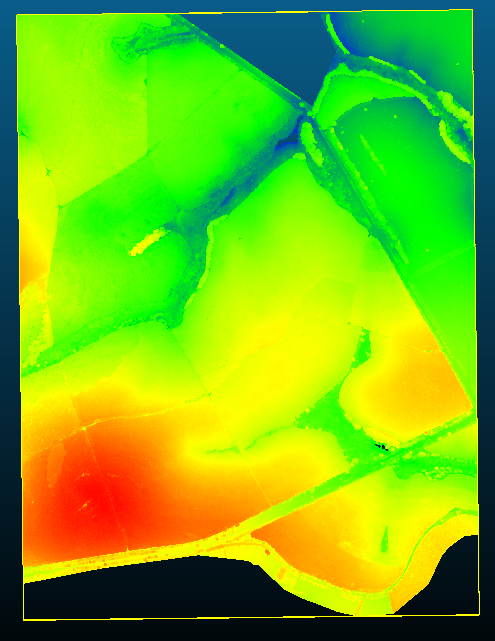
\includegraphics[width=0.4\linewidth]{IMAGES/pre-clipagem-passo8} 

}

\caption{Nuvens de pontos LiDAR pré-processadas}\label{fig:unnamed-chunk-8}
\end{figure}

\begin{enumerate}
\def\labelenumi{\roman{enumi}.}
\setcounter{enumi}{1}
\tightlist
\item
  As nuvens foram baixadas pelo seguinte link:
  \url{https://github.com/FlorestaR/dados/blob/main/5_LIDARF/Modelo/CLOUDS/}
\end{enumerate}

\newpage
6

. Download e leitura dos dados em Shapefile\\
i. Os shapes foram baixados pelo seguinte link:
\url{https://github.com/FlorestaR/dados/blob/main/5_LIDARF/Modelo/SHAPES}

\begin{figure}

{\centering 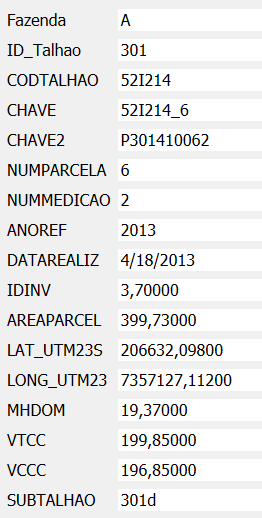
\includegraphics[width=0.5\linewidth]{IMAGES/atributosinventariadas} 

}

\caption{Dados contidos nas parcelas inventariadas}\label{fig:unnamed-chunk-9}
\end{figure}

\newpage
7

. Clipagem da nuvem para eliminação de dados indesejados (mostrar nuvem
antes e depois)\\
Antes da clipagem: 68mi pontos\\
Após clipagem: 18mi pontos

\begin{figure}

{\centering 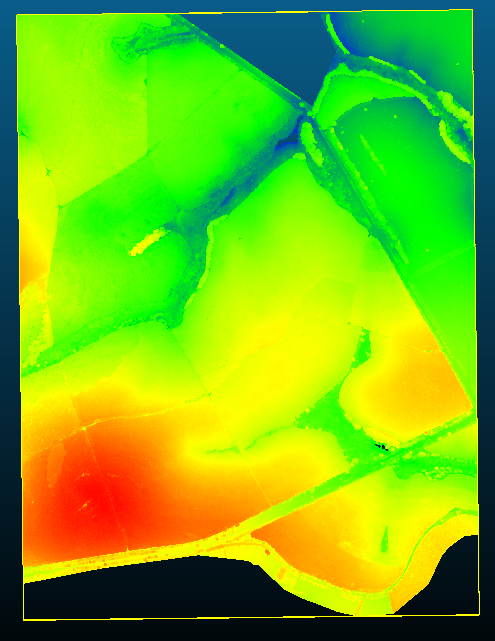
\includegraphics[width=0.4\linewidth]{IMAGES/pre-clipagem-passo8} 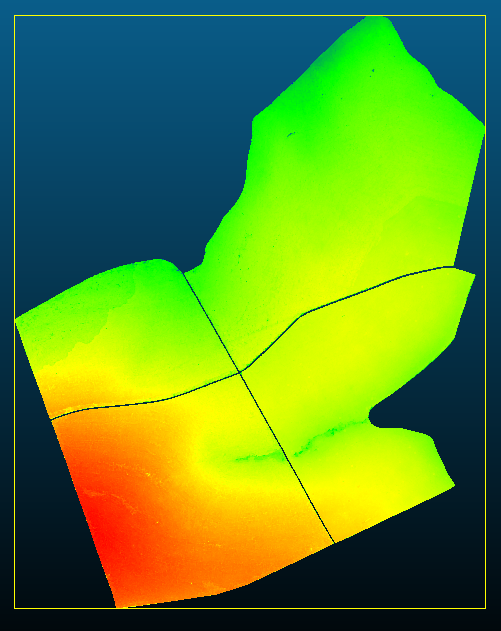
\includegraphics[width=0.4\linewidth]{IMAGES/pos-clipagem-passo8} 

}

\caption{Comparativo entre as nuvens de pontos antes e após a clipagem}\label{fig:unnamed-chunk-10}
\end{figure}
\newpage
8

. Classificação

\begin{figure}

{\centering 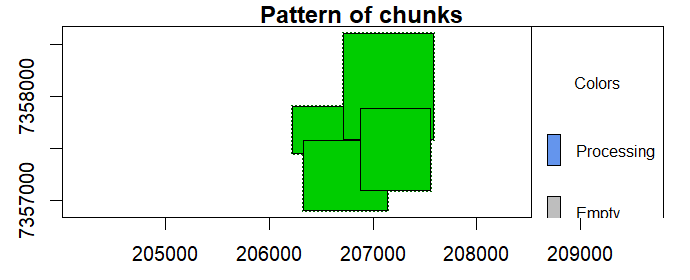
\includegraphics[width=0.4\linewidth]{IMAGES/classificacao-pontos-de-solo} 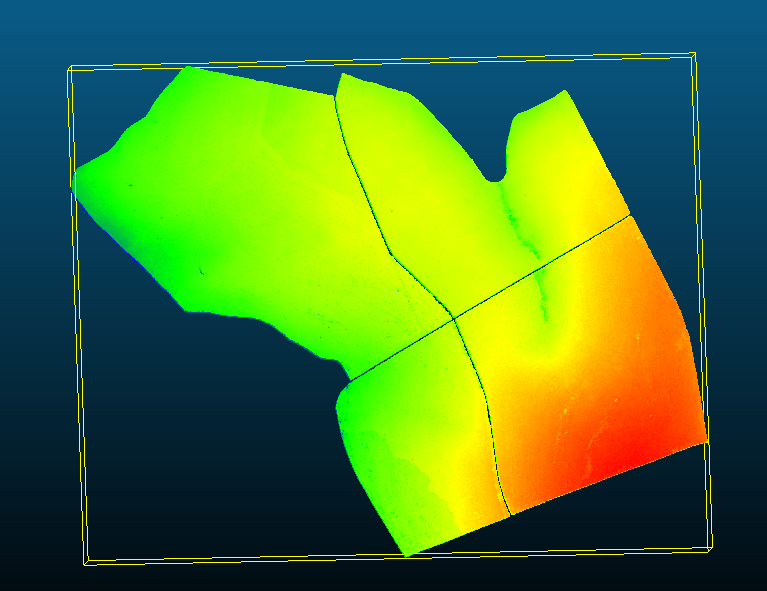
\includegraphics[width=0.4\linewidth]{IMAGES/nuvem-com-pontos-de-solo-classificados-mas-sem-normalizacao} 

}

\caption{Processamento e resultado da classificação de solo das nuvens LiDAR}\label{fig:unnamed-chunk-11}
\end{figure}
\newpage
9

. Normalização i. A etapa de normalização tem por finalidade nivelar
toda a nuvem e é um passo que está diretamente correlacionado à
classificação do solo.

\begin{figure}

{\centering 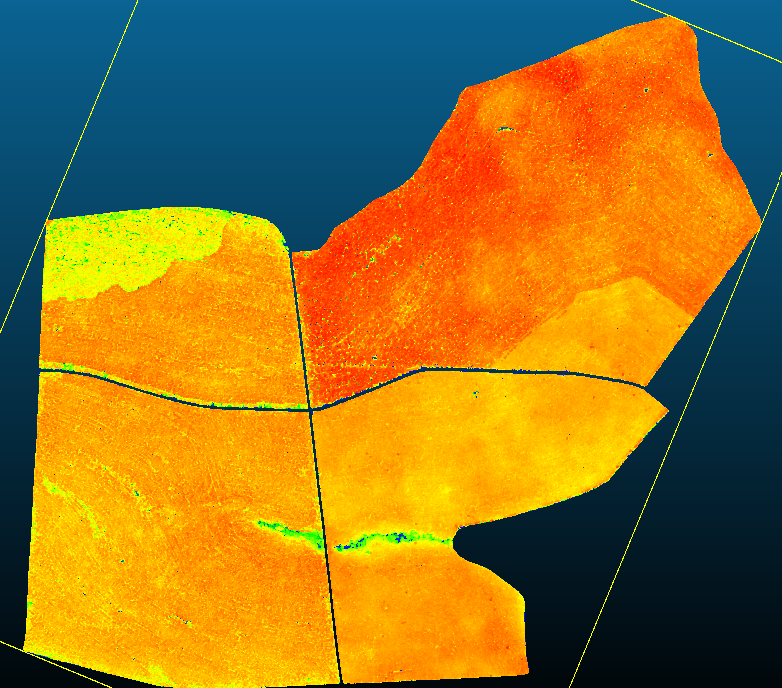
\includegraphics[width=0.4\linewidth]{IMAGES/nuvensnormalizadas} 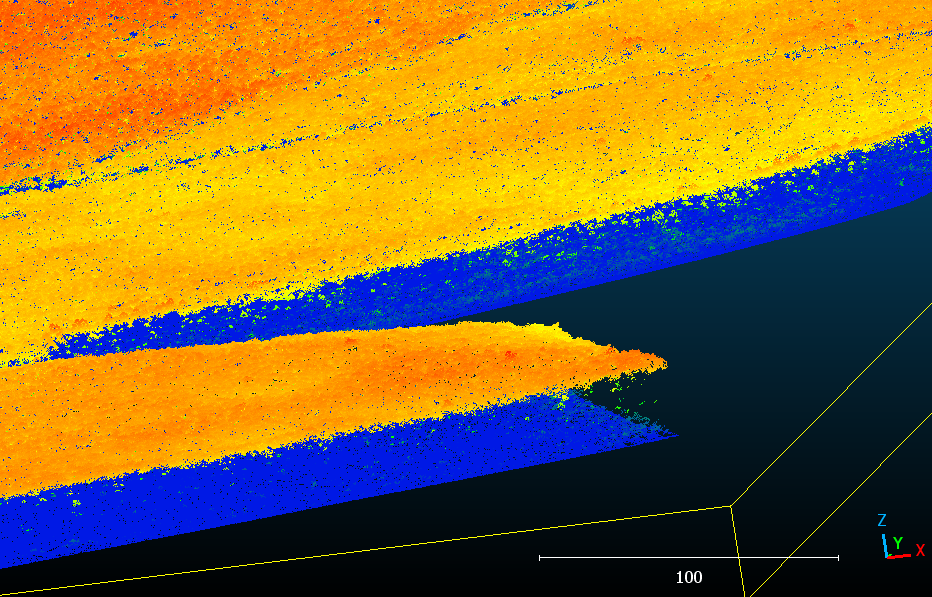
\includegraphics[width=0.4\linewidth]{IMAGES/nivelamento} 

}

\caption{Resultado da normalização das nuvens}\label{fig:unnamed-chunk-12}
\end{figure}
\newpage
10

. Recorte da nuvem em tiles 300x300m O recorte da nuvem em tiles menores
tme a função de facilitar o processamento dos dados, tornando-o mais
rápido e dinâmico

\begin{figure}

{\centering 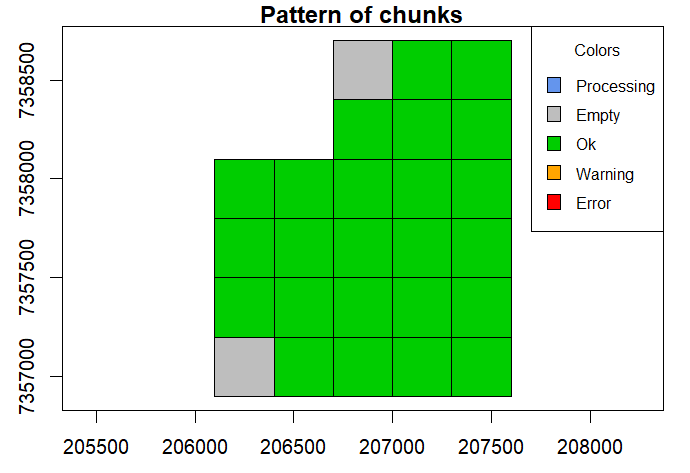
\includegraphics[width=0.5\linewidth]{IMAGES/Retile} 

}

\caption{Retile da nuvem em quadrados de 300x300m}\label{fig:unnamed-chunk-13}
\end{figure}
\newpage

\begin{enumerate}
\def\labelenumi{\arabic{enumi}.}
\setcounter{enumi}{10}
\tightlist
\item
  Cálculo de métricas para cada voxel (explicar voxel)
\end{enumerate}

\begin{figure}

{\centering 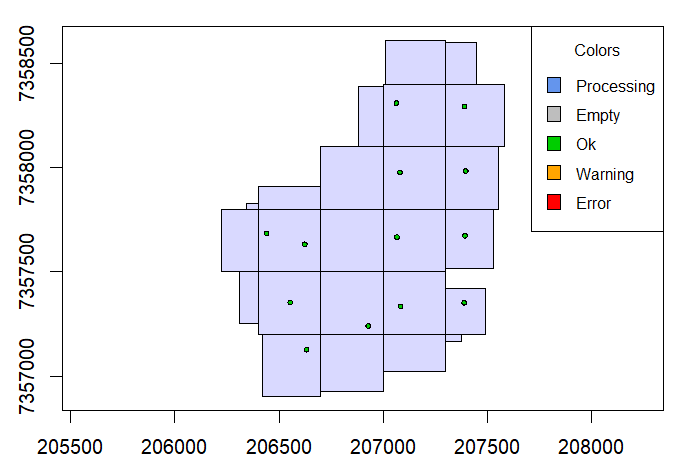
\includegraphics[width=0.5\linewidth]{IMAGES/calculo-metricas-voxel} 

}

\caption{Cálculo das métricas para cada voxel}\label{fig:unnamed-chunk-14}
\end{figure}
\newpage
12

. Seleção de um grupo de métricas para estudo de correlação

\begin{figure}

{\centering 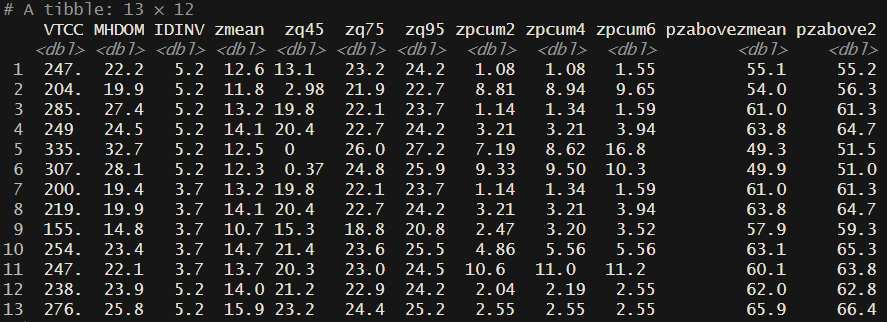
\includegraphics[width=0.5\linewidth]{IMAGES/tb-subgrupo-de-metricas-p-analise} 

}

\caption{Tabela com as métricas escolhidas}\label{fig:unnamed-chunk-15}
\end{figure}
\newpage
13

. Análise da correlação por meio de gráfico (falar do gráfico)

\begin{figure}

{\centering 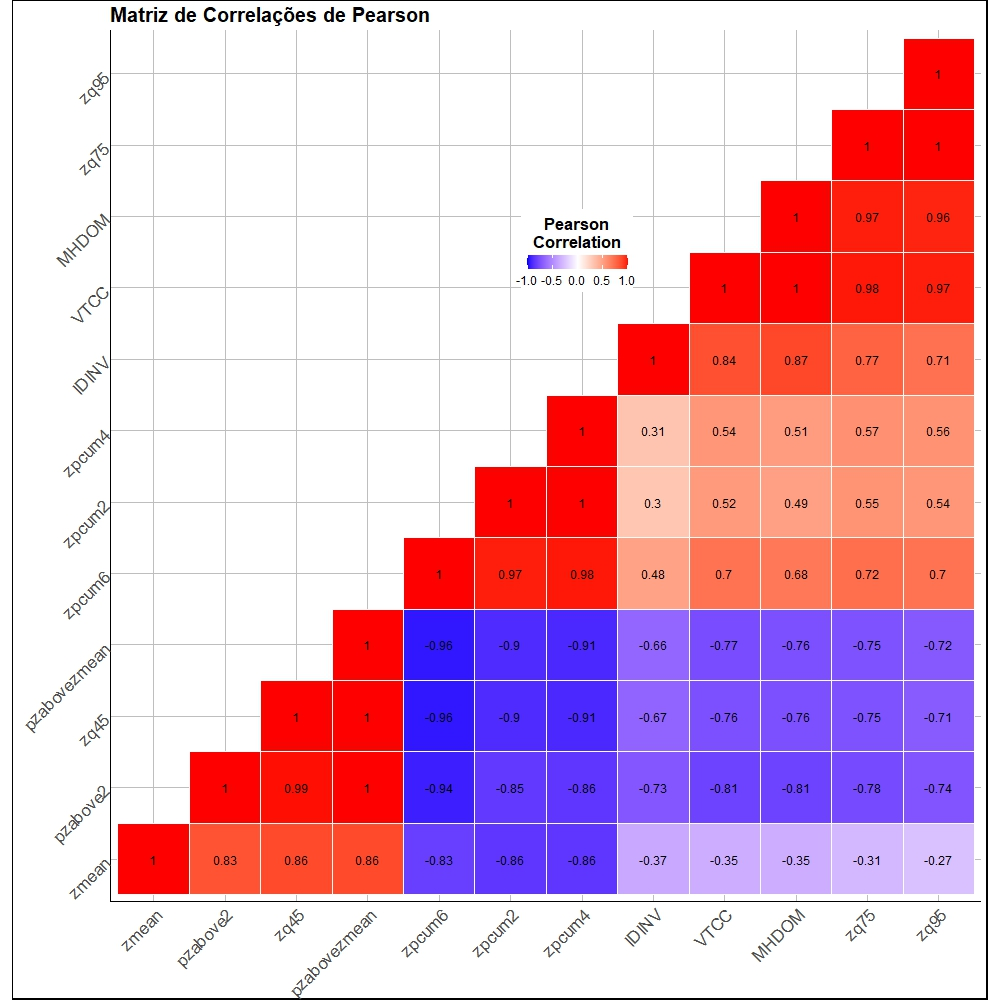
\includegraphics[width=0.5\linewidth]{IMAGES/MatrizDeCorrelacoes} 

}

\caption{Resultado da análise de correlação}\label{fig:unnamed-chunk-16}
\end{figure}
\newpage
14

. Determinação do modelo de predição

\begin{figure}

{\centering 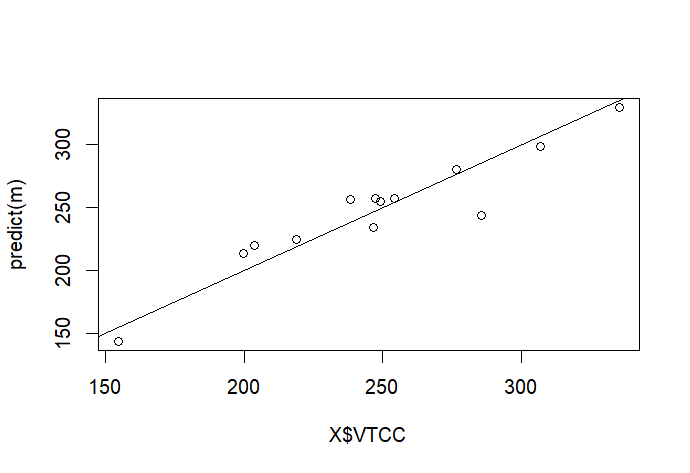
\includegraphics[width=0.5\linewidth]{IMAGES/analise-de-regressao} 

}

\caption{nao sei}\label{fig:unnamed-chunk-17}
\end{figure}
\newpage
15

. Criação de mapas raster e gráficos \newpage

\end{document}
